\documentclass[12pt,onecolumn,a4paper]{article}
\usepackage{epsfig,amsthm,amsmath,booktabs,csquotes}
\usepackage [pagebackref=true, colorlinks, linkcolor=blue, citecolor=magenta, urlcolor=cyan] {hyperref}
\usepackage{color,xcolor}

\usepackage{titlesec} %include more subsection than subsubsection

\usepackage{subcaption}
\usepackage[labelformat=parens,labelsep=quad, skip=3pt]{caption}
\usepackage{graphicx}
\usepackage{enumerate,braket,tcolorbox}
\usepackage[localise]{xepersian}
%\settextfont[Scale=1.2]{‌BNAZANIN.TTF}
%\settextfont[Scale=1.2]{BZAR.TTF}
\settextfont[Scale=1]{XB Niloofar}
\ExplSyntaxOn
\cs_set_eq:NN
\etex_iffontchar:D
\tex_iffontchar:D
\cs_undefine:N \c_one
\int_const:Nn \c_one { 1 }
\ExplSyntaxOff
\setdigitfont[Scale=1]{XB Niloofar}
\setlatintextfont[Scale=1]{Times New Roman}

% set local changes to margin
\def\changemargin#1#2{\list{}{\rightmargin#2\leftmargin#1}\item[]}
\let\endchangemargin=\endlist 
%

% newcommands
\newcommand{\floor}[1]{\left\lfloor #1 \right\rfloor}
\newcommand{\ceil}[1]{\left\lceil #1 \right\rceil}

\begin{document}
\title{مطالعه همگامی در شبکه‌های عصبی} 
\author{محسن مهرانی - استاد راهنما: دکتر سامان مقیمی عراقی}
\date{}
\maketitle
\tableofcontents
\newpage
\قسمت{سخن نخست}
مطالعه فعالیت شبکه‌های عصبی برای تحقیق و بررسی کارکردهای مغز اهمیت زیادی دارد. همه بر این باوریم که مغز محمل اندیشه و تفکر است. ما کنجکاو هستیم که چگونه همکاری بین نورون‌های آن باعث می‌شود تا حافظه، کشف و پردازش صورت گیرد. هر کدام از نورون‌های مغز می‌تواند در حالت فعال [روشن] یا غیرفعال [خاموش] قرار گیرد. هم اکنون شواهدی وجود دارد که کارکردهایی طلایی یاد شده مغز در زمان‌هایی رخ می‌دهند که الگوی خاموش و روشن شدن نورون‌های آن باهم \textbf{«هم‌گامی»} دارند. هم‌گامی به این معناست که جمعیت بزرگی از نورون‌ها هم باهم خاموش و روشن می‌شوند و یک الگوی تکرار شونده‌ای را دنبال می‌کنند. تو گویی که باهم هم‌آهنگ یا هم‌گام شده‌اند.\\

بی‌تردید دستیابی به تمام جزییات مغز برای ما میسّر نیست و به آن به عنوان یک \textbf{«جعبه‌ی سیاه»} نگاه می‌کنیم که مدت‌هاست به دنبال ارائه مدلی هستیم که رابطه‌ی بین ورودی‌ها و خروجی‌های ثبت شده را بازتولید کند. کاری که در این پژوهش انجام خواهیم داد تلاشی است برای پیشنهاد دادن یک مدل برای این جعبه‌ی سیاه که رفتار نسبتا مشابهی را میان ورودی و خروجی‌های این جعبه سیاه و یا مغز ایجاد می‌کند.

\قسمت{مقدمه}
مدل‌های زیادی برای شبکه‌های عصبی ارائه شده است که توانایی تولید رفتار هم‌گام شدن نورون‌ها را در آن‌ها می‌توانیم جستجو کنیم. یکی از این مدل‌ها که در تمام فصول شبیه‌سازی از آغاز تا کنون از آن بهره برده شده است؛ مدل انباشت و شلیک است\cite{PhysRevLett.105.158104}. در این جستار ابتدا با مدل انباشت و شلیک شروع می‌کنیم و سپس مدلی توسعه یافته که آن را \textbf{«چرخنده»} صدا خواهیم کرد؛ می‌پردازیم.\\
متن اصلی این جستار شامل معرفی این مدل‌ها و پویایی آن‌ها در زمان و نتایج ضبط شده از نشانگرهایی است که برای آشکارسازی هم‌گامی تعبیه شده‌اند.

\قسمت{شبکه انباشت و شلیک}
 در این نوشتار \cite{PhysRevLett.105.158104}  نویسندگان تلاش می‌کنند تا هم‌گامی را برای شبکه‌ی نورون‌های مهاری رصد کنند. این نورون‌ها به گونه‌ای باهم مرتبط هستند که تیزه زدن هر نورون منجر به مهار پتانسیل دیگر نورون‌ها می‌شود. تک‌تک نورون‌های این شبکه از تحول انباشت و شلیک تبعیت می‌کند. معادله تحول اختلاف پتانسیل هر کدام از نورون‌ها با محیط بیرونش از رابطه زیر داده می‌شود:
 \begin{tcolorbox}
\begin{align}
\dot{v_i}=a_i - v_i - \frac{g}{N} \sum_{n|t_n<t} S_{i,l(n)} \delta(t - t_n - t_d) 
\label{eq:potential_1}
\end{align}

\begin{enumerate}[-]
\item
$g$: 
ضریب اتصال هر جفت نورون. از آن‌جا که همه‌ی نورون‌ها در این مطالعه مهاری هستند؛ باید این کمیت مثبت انتخاب شود تا تاثیر جمله‌ی پایانی در نهایت منفی باشد.
\item
$S$:
ماتریس همسایگی. این کمیت نشان می‌دهد که آیا دو نورون به هم متصل و تاثیرگذار هستند یا خیر.
\item
$t_d$: 
زمان تاخیر میان زدن تیزه هر نورون و تاثیر آن روی نورون‌های دیگر.
\item
$a_i$:
یک پتانسیل تحریکی و خارجی. در این مطالعه این مقدار برای هر نورون به صورت تصادفی انتخاب می‌شود و تا پایان شبیه‌سازی ثابت باقی می‌ماند.
\item
$N$:
تعداد نورون‌های در شبکه
\end{enumerate}
\end{tcolorbox}
\زیرقسمت{آهنگ تیزه زدن}
پیش از آن که به شبیه‌سازی یک شبکه‌ از نورون‌ها بپردازیم؛ خوب است تا یک نورون تنها را مطالعه کنیم. یک نورون تنها که پویایی از جنس مدل انباشت‌وشلیک دارد؛ دوره تناوب تیزه‌زدن آن از رابطه‌ی زیر قابل محاسبه است .
\begin{align}
\dot{v_i}= I  - v_i &\rightarrow \frac{dv_i}{I - v_i} = dt \\
&\rightarrow T = ln(\frac{I}{I - 1})
\end{align}
این رابطه نشان می‌دهد که بسامد تیزه‌زدن یک نورون با افزایش مجموع جریان‌های ورودی آن به صورت لگاریتمی افزایش می‌یابد.
\زیرقسمت{نشانگر تشخیص فاز هم‌گامی}
برای آن که متوجه شویم که شبکه در حالت هم‌گامی یا ناهم‌گامی است نیاز است تا آشکارسازی را تعبیه کنیم که باتوجه به رفتار سامانه، هم‌گامی یا ناهم‌گامی را با عقربه‌ی خود نشان دهد. برای این منظور ابتدا مفهوم میدان ($E$) را تعریف می‌کنیم که بیانگر شدت فعالیت نورون‌های شبکه است. انحراف از معیار این کمیت در طول زمان، پارامتر مناسبی است که به کمک آن هم‌گامی را تشخیص دهیم.
\begin{tcolorbox}
\begin{align}
\ddot{E}+ 2\alpha \dot{E}+\alpha^{2}E &=\frac{\alpha^2}{N} \sum_{n|tـn<t} \delta(t - t_n - t_d) \\
\sigma^{2} &= \braket{E^{2}}_{t} - \braket{E}^{2}_{t}
\end{align}
*دقت کنیم که شدت میدان با تعداد تیزه زدن‌ها رفتاری ملایم دارد. به عنوان مثال اگر تیزه‌ها متوقف شوند؛ شدت میدان پس از لحظاتی چند [متناسب با $\alpha$] صفر می‌شود.
\end{tcolorbox}

در طول زمان میدان $E$ و $\sigma$ را رصد می‌کنیم. برای دریافت شهودی عملکرد مناسب این پارامتر نظم، فرض کنید که شبکه در حالتی است که جمعیت بزرگی از آن در حال خاموش و روشن شدن هم‌گام است. پس مشاهده خواهم کرد که میدان که شدت فعالیت نورون‌ها را نشان می‌دهد در حال ضربان رفت و برگشتی است. این افت‌وخیز با تقویت هم‌گامی دامنه‌ی بزرگتر پیدا می‌کند به طوری که انحراف آن از میانگین پهنای قابل توجهی کسب می‌کند. از این رو انحراف معیار میدان، کمیت مناسبی است که میزان هم‌گامی را گزارش کند.\\

\subsection{مسائل پیشروی پیاده سازی شبیه سازی}
\subsubsection{تابع بی‌کران دلتا}
یکی از مشکلات شبیه سازی معادلات دیفرانسیلی حضور تابع دلتای دیراک است. این تابع در نقطه صفر خود دارای مقداری بینهایت است. معرفی چنین تابعی به رایانه کاری دشوار است و همانندی محاساتی ندارد. حال برای برطرف کردن این مشکل چه باید کرد؟ نکته در این جا نهفته است که چون ما برای حل عددی معادله دیفرانسیلی خود از زمان پیوسته استفاده نمی‌کنیم و از گام‌هایی با طول مثبت $\Delta t$ استفاده می‌کنیم این مشکل به صورت زیر مدیریت می‌شود.
\begin{align}
v_{i}(t+\Delta t) &= v_{i}(t) + \int_{t}^{t+\Delta t} \dot{v_i}  dt \\
&= v_{i}(t) + \int_{t}^{t+\Delta t} \left[ a_i - v_i - \frac{g}{N} \sum_{n|t_n<t} S_{i,l(n)} \delta(t - t_n - t_d)  \right]   dt \\
&\approx v_{i}(t) +  \left[ a_i - v_i(t) \right] \Delta t - \frac{g}{N} \sum_{n|t_n<t} S_{i,l(n)} \int_{t}^{t+\Delta t} \delta(t - t_n - t_d) dt  \\
&\approx v_{i}(t) +  \left[ a_i - v_i(t) \right] \Delta t - \frac{g}{N} \sum_{n|t_n<t} S_{i,l(n)} H(t + \Delta t- t_n - t_d) \label{eq:potential_changes}
\end{align}

حالا تابع پله کاملا برای ما آشنا و قابل مدلسازی است. دقت شود که تابع پله یاد شده فقط در محدوده $t, t+\Delta t$ زندگی می‌کند و پس از آن اعتبار ندارد. معادله \ref{eq:potential_changes}  می‌گوید که باید برای تحول پتانسیل نورون $i$ام بررسی کنیم که آیا نورونی در همسایگی آن تیزه زده است یا نه. اگر چنان باشد؛ یک واحد به جمع تیزه زدگان اضافه کنیم.


\subsubsection{ثبت تاریخ تیزه زدن‌ها}
برای محاسبه تحول پتانسیل در رابطه \ref{eq:potential_changes} چنان که توضیح داده شد نیاز به دانستن تاریخ تیزه زدن‌ها داریم. اگر بخواهیم برای تمامی نورون‌ها در هر گام زمانی تیزه‌زدن آن را به صورت مجزا ثبت کنیم؛یک آرایه مربعی خواهیم داشت که شماره سطر آن می‌تواند معرف زمان باشد و ستون نماد شماره نورون - شکل شماره (\ref{fig:rasterplot}).\\
\begin{figure}[h]
\centering
  \includegraphics[width = 10 cm]{../scripts/kuramoto_model_synchoronization_problem/single_runs/N1000_T1000_g5_input_1.2_2.8/raster_plot.png}
 \caption{ثبت لحظه‌ای تیزه زدن هر نورون به صورت مجزا - در این نمودار ضریب تاثیر هر نورون روی همسایه‌هایش $g = 5$ بوده است. چنان که انتظار می‌رفت شاهد هم‌گامی هستیم.}
  \label{fig:rasterplot}
\end{figure}
اما مشکلی که برای این شبیه سازی رخ خواهد داد. در صورت افزایش تعداد نورون‌ها و زمان شبیه سازی با یک ابر آرایه روبرو خواهیم شد که امکان دارد در ذخیره سازی آن دچار مشکل شویم. به همین خاطر در شبیه سازی انجام شده تنها مجموع تیزه زدن‌ها را ذخیره کردیم تا یک آرایه یک ستونه داشته باشیم و در ذخیره‌سازی به مشکل نخوریم.

\subsection{نتایج}
اندازه‌ی پارامتر‌هایی که برای این شبیه‌سازی انتخاب کردیم؛ کاملا از صورت مقاله یاد شده برداشته شده و به قرار زیر است.
\begin{tcolorbox}[colback=green!5!white,colframe=green!75!black]
\begin{enumerate}[*]
\item
$\alpha = 20\, s^{-1}$
\item
جریان‌های تصادفی خارجی نورون‌ها از اعضای بازه‌ی $(1.2,2.8)$ انتخاب می‌شوند.
\item
$N = 10000$
\item
$t_d = 0.1\, s$ 
\end{enumerate}
\end{tcolorbox}
این شبیه سازی برای ۱۰۰۰ ثانیه اجرا شده است که در آن هر گام زمانی برابر $0.01$ ثانیه گرفته شده است. کد شبیه‌سازی در پوشه 
\href{run://..//scripts//kuramoto_model_synchoronization_problem}{مسئله همگامی برای مدل انباشت‌و‌شلیک}
قابل مشاهده است.
\زیرزیرقسمت{انحراف از معیار میدان}
مهم‌ترین شاخصه ما برای ردگیری همگامی، انحراف معیار میدان $E$ است که با زیگما $\sigma$ نمایش می‌دهیم. جهش به وجود آمده در شکل‌ (\ref{fig:if_phase_transition}) به این معنی است که سامانه از حالت ناهم‌گامی به هم‌گامی تغییر فاز داده است. 

\begin{figure}[h]
\centering
  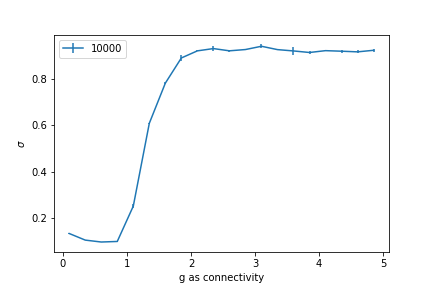
\includegraphics[width = 10 cm]{../papers_studies/figs/IF/sigma.png}
 \caption{تغییر فاز از ناهم‌گامی به هم‌گامی برای ۱۰۰۰ نورون}
  \label{fig:if_phase_transition}
\end{figure}

\زیرزیرقسمت{نورون‌های خاموش}
بی‌تردید میدان داخلی نورون‌ها کاملا تابعی است از آمارتیزه‌های درون سامانه. نورون‌هایی که گاهی برای تیزه زدن به پیش می‌روند و گاه به علت حضور میدان داخلی مهار به عقب برمی‌گردند. خوب است بپرسیم که برآیند این رفت و برگشت‌ برای هر نورون چگونه است. آیا این رفت و برگشت منجر به رسیدن به آستانه‌ی تیزه زدن می‌شود و یا نورون در برآیند اصلا پیشروی نمی‌کند و هیچگاه به آستانه نمی‌رسد و خاموش می‌ماند.\\
در شکل \ref{fig:if_silent_neurons} شمار نورون‌هایی که هیچگاه در سامانه تیزه نمی‌زنند را آورده‌ایم و این که چگونه با با افزایش ضریب تاثیر مهاری میدان این آمار رشد می‌کند.\\
این مشاهده نشان می‌دهد که در فاز هم‌گام، تقریبا ۲۵ درصد نورون‌ها خاموش هستند و نقشی در برقراری جریان داخلی ندارند. قابل حدس است که نورون‌هایی خاموش هستند که جریان‌های تصادفی خارجی پایین دست را داشته‌اند. به این معنی که اگر بازه‌ی جریان تصادفی را تنگ‌تر می‌گرفتیم [ مثلا از$1.6$ ] شروع می‌کردیم؛ سامانه در فاز هم‌گام تفاوت رفتاری نمی‌داشت.\\
همچنین جالب است که تغییر فاز مشاهده شده در تعداد نورون‌های خاموش - شکل \ref{fig:if_silent_neurons}-در حالتی در همسایگی و متمایز از تغییر فاز شکل \ref{fig:if_phase_transition} نشان می‌دهد.
\begin{figure}[h]
\centering
  \includegraphics[width = 10 cm]{../scripts/all_neurons_model_in_one_place/IF_ensembles/N10000_T1000_I1.2_2.8_cluster_computed/silent_neurons_g_0.1_65.png}
 \caption{آمار نورون‌های خاموش درون سامانه}
  \label{fig:if_silent_neurons}
\end{figure}

\زیرزیرقسمت{توزیع تناوب زمانی تیزه‌ها}
شبکه‌ی ما متشکل از نورون‌هایی است که مدام در حال تیزه زدن و فعال نگه‌داشتن شبکه هستند. برخی با بسامد بیشتری تیزه می‌زنند و برخی آهسته‌تر. اگر کنجکاو باشیم که جمعیت کل نورون‌های ما چگونه میان دسته‌های مختلف با تناوب‌های متفاوت توزیع شده‌ است؛ لازم است تا توزیع فراوانی آن‌ها را یکجا رسم کنیم - شکل \ref{fig:if_isi}.\\
همان طور که می‌بینید به ظاهر این توزیع رفتاری توانی دارد و اگر کنجکاو باشیم می‌توانیم شیب این نمودار تمام لگاریتمی آن را جهت محاسبه‌ی نمای توزیع بدست آوریم - شکل \ref{fig:if_isi_trending_line}.
\begin{figure}[h]
\centering
  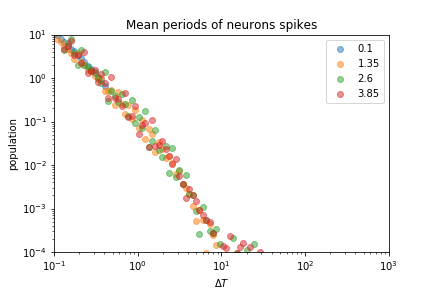
\includegraphics[width = 10 cm]{../papers_studies/figs/IF/mean_spiking_persiods.png}
 \caption{توزیع بسامدی شبکه‌های ۱۰۰۰ نورونی که هر کدام قدرت اتصال متفاوتی دارند. }
  \label{fig:if_isi}
\end{figure}

\begin{figure}[h]
\centering
  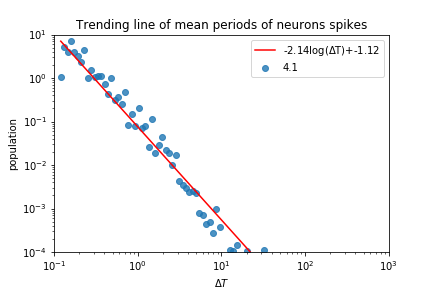
\includegraphics[width = 10 cm]{../papers_studies/figs/IF/mean_spiking_persiods_with_trending_line.png}
 \caption{محاسبه‌ی نمای توزیع توانی فاصله زمانی بین تیزه‌ها}
  \label{fig:if_isi_trending_line}
\end{figure}

\زیرقسمت{پهن‌کردن قالی صفحه‌ی فاز}
در قسمت‌های پیشین تنها به مطالعه‌ی تاثیر ضریب اتصال در تغییرفاز پرداختیم و زمان تاخیر را تنها در $t_d = 0.1 s$ خلاصه کردیم. حال اجازه دهید تا به تاخیر نیز اجازه‌ی تغییر دهیم. در ادامه‌ی این قسمت از نوشتارمان، به فرش‌کردن صفحه‌ی فاز خود خواهیم پرداخت. امید است که چهره‌ی تمام نمای سامانه‌ بر صورت این قالی نقش بندد.\\


\زیرزیرقسمت{قالی انحراف از معیار میدان}
در شکل \ref{fig:if_g_d_phase_space} مشاهده می‌کنیم که شدت هم‌گامی در هر کدام از هنگردهای سامانه چقدر است. بنظر می‌رسد که با افزایش زمان تاخیر و ضریب تاثیر همگامی قدرت پیدا می‌کند و هر دو در ظهور این رفتار شریک هستند. اگر چه تاخیر در جابجایی ضریب‌تاثیر بحرانی تغییری ایجاد نکرده است اما هم‌گامی را قدرت می‌بخشد.
\begin{figure}[h]
\centering
  \includegraphics[width = 15 cm]{../scripts/all_neurons_model_in_one_place/IF_ensembles/N10000_T1000_I1.2_2.8_cluster_computed/sigma_phase_space.png}
 \caption{صفحه‌ی فاز مربوط به سامانه‌ی نورون‌های انباشت‌وشلیک}
  \label{fig:if_g_d_phase_space}
\end{figure}
%\زیرزیرقسمت{قالی دوره‌تناوب غالب}



\section{شبکه‌ی نورون‌های چرخنده}
در این مدل به جای آن که برای شبکه خود از مدل انباشت-شلیک استفاده کنیم از مدل چرخنده استفاده می‌کنیم. در این مدل نورون‌های ما مانند دونده‌هایی به دور میدان مثلثاتی می‌دوند. ما نقطه‌ی فاز $\pi$ را به عنوان علامت برای این دونده‌ها قرار دادیم. هر زمان که دونده‌ای از علامت خود گذشت یک تیزه برای او درنظرمی‌گیریم و بلافاصله او را به فاز $-\pi$ باز می‌گردانیم.\\

برای توصیف فاز هر نورون از معادلات زیر استفاده می‌کنیم:
\begin{tcolorbox}
\begin{equation}
\begin{cases}
\dot{\theta_i}=I_i - cos(\theta_i) - g E, \hspace{2ex} - 5\pi/2 \leq \theta_i \leq \pi \\
\dot{E} = M - \alpha E\\
\dot{M} = -  \alpha M + \frac{ \alpha^{2} }{N} \sum_{n|tـn<t} \delta(t - t_n - t_d)
\end{cases}
\end{equation}
\begin{enumerate}[-]
\item $\theta_i$:
مشخص کننده‌ی فاز هر نورون. این فاز میان دو لبه در حال حیات است. کوچکترین کران بالای آن همان حالت آستانه در $\pi$ است و بزرگترین کران پایین آن نگه‌دارنده‌ای است که از ریزش نورون‌ها جلوگیری می‌کند.
\item $E$:
میدانی است که شدت فعالیت شبکه را نشان می‌دهد.
\item $M$:
یک پارامتر فرعی که در حل معادله دیفرانسیل مرتبه دوم به دو معادله‌ی تحول مرتبه اول ما را یاری کرده است.
\end{enumerate}
\end{tcolorbox}

این مدل نسبت به مدل قبلی شامل ویژگی‌های مثبتی است. یکی از ویژگی‌های خوب آن این است که پس از بازنشانی فاز نورون تیزه زده، فاز آن به زاویه‌ای برده می‌شود که دارای خواص مثلثاتی مشابهی است. به این معنا که دیگر شاهد گسستگی در اندازه‌ی جملاتی که تحول نورون را توصیف می‌کنند؛ نیستیم.\\
\زیرقسمت{آهنگ تیزه زدن}
برای نورونی تنها که پویایی از جنس چرخنده دارد؛ دوره‌ی تناوب تیزه زدن آن بر حسب مجموع جریان ورودی‌ رفتاری مطابق زیر دارد \cite{safaeesirat2020critical}:

\begin{align}
T = \frac{2\pi}{\sqrt{I^2 - 1}}
\end{align}
این به این معناست که مدل چرخنده و انباشت‌وشلیک اگر چه هر دو با افزایش جریان، بسامد تیزه زدنشان افزایش می‌یابد اما رفتار تغییر آن به دو گونه‌ی متفاوت صورت می‌پذیرد. این نکته‌ی مهمی است که در هنگام مقایسه‌ی دو مدل باید به خاطر داشته باشیم.

\زیرقسمت{نشانگر توسعه یافته‌ی تشخیص همگامی}
برای تشخیص هم‌گامی از یک پارامتر دیگری که در این مقاله \cite{safaeesirat2020critical}  توسط نویسندگان ابداع شده‌است؛ بهره می‌بریم.

\begin{equation}
s =  \braket{ \big[ \frac{1}{N_a}\sum_{i_a} sin(\theta_{i_a}) \big]^{2}}_t
\label{eq:saman_amin_param}
\end{equation}
میانگین‌گیری بالا روی ۱۰۰۰ گام آخر زمانی انجام می‌شود. این فاصله زمانی باید حتما بزرگ‌تر از گام‌های زمانی تحول ریزمقیاس آن باشد. همچنین برای این متوسط‌گیری نورون‌هایی را مدنظر می‌گیریم که در منطقه ی فعال قرار گرفته‌اند. منطقه‌ی فعال، سمت چپ دایره مثلثاتی است.
\subsection{شبیه‌سازی}
ثوابت مسئله را به گونه‌ی زیر انتخاب می‌کنیم.
\begin{tcolorbox}[colback=green!5!white,colframe=green!75!black]
\begin{enumerate}[*]
\item
$\alpha = 20\, s^{-1}$
\item
جریان‌های تصادفی خارجی نورون‌ها از اعضای بازه‌ی $(9.5,13.5)$ انتخاب می‌شوند. این بازه به گونه‌ای انتخاب شده است که نورون خاموشی در سامانه وجود نداشته باشد.
\item
$N = 10000$
\item
$t_d = 0.1\, s$ 
\end{enumerate}
\end{tcolorbox}
حال شبکه‌ی خود را به ازای قدرت اتصال‌های مختلف اجرا می‌کنیم تا مجددا تحقیق کنیم که چگونه تغییر در قدرت اتصال $g$ می‌تواند باعث شود تا تغییر فاز از ناهم‌گامی به هم‌گامی رخ دهد. برای مشاهده‌ی دفترچه شبیه‌سازی به آدرس 
\href{run://..//scripts//rotational_model}{مسئله همگامی برای مدل چرخنده}
مراجعه کنید.

\subsection{نتایج }
مرتبه‌ی اجرای این الگورتیم خطی است و برای یک شبکه شامل ۱۰۰۰ نورون و برای ۱۰۰۰۰ گام شبیه‌سازی زمانی در حدود ۴ ثانیه به طول می‌انجامد. 


\subsubsection{در جستجوی تغییرفاز}
پس از رصد کردن تغییرات رفتار سیستم بر حسب قدرت مهار نورون‌ها، تغییر فاز مانند مدل قبلی مشاهده شد اما مکان تغییر فاز تغییر کرد و حول $g=30$ قرارگرفت. این تغییر فاز در دو شکل \ref{fig:sigma_rotational} و \ref{fig:amin_saman_rotational}  قابل مشاهده‌است.
\begin{figure}
\centering
  \includegraphics[width = 10 cm]{../scripts/all_neurons_model_in_one_place/Rotational_ensembles/N10000_T100_I9.5_13.5_cluster_computed/sigma_g_0.1_65.png}
 \caption{پهنای جریان یک سامانه چرخنده با ده هزار نورون}
  \label{fig:sigma_rotational}
\end{figure}

\begin{figure}
\centering
  \includegraphics[width = 10 cm]{../scripts/all_neurons_model_in_one_place/Rotational_ensembles/N10000_T100_I9.5_13.5_cluster_computed/amin_saman_param_g_0.1_65.png}
 \caption{پارامتر نظم تعریف شده در رابطه \ref{eq:saman_amin_param} برای مدل چرخنده }
  \label{fig:amin_saman_rotational}
\end{figure}


\subsubsection{فاصله زمانی بین تیزه‌ها}
حال که دیدیم برخی نورون‌ها همواره خاموش می‌مانند و یا به عبارتی دوره‌ی تیزه زدن آن‌ها بینهایت است؛ خوب است که دوره‌ی تیزه زدن‌های نورون‌های دیگر را نیز بررسی کنیم. شکل \ref{fig:interspikes_rotational} این شکل نمایان‌گر آن است که توزیع دوره‌ها به توزیع بی‌توانی و رفتار بی‌مقیاس نزدیک است.\\
همچنین توجه کنیم که با افزایش ضریب تاثیر رفتار توانی آن‌ها تغییر نمی‌کند. تنها تفاوت در چگونگی انتخاب جایگاه‌های روی خط است. هر چه ضریب تاثیر بزرگتر می‌شود نورون‌ها فاصله‌ی زمانی تیزه‌های بزرگتری را اتخاذ می‌کنند.
\\
با این مشاهده، کنجکاو می‌شویم تا نمای بحرانی را برای آن حساب کنیم. در شکل \ref{fig:interspikes_rotational_trending_line} با گذراندن یک خط بر داده‌های بدست آمده از شبکه‌ای با قدرت مهار ۲۰ را می‌بینیم.

\begin{figure}[h]
\centering
  \includegraphics[width = 10 cm]{../scripts/all_neurons_model_in_one_place/Rotational_ensembles/N10000_T100_I9.5_13.5_cluster_computed/mean_spiking_persiods_g_0.1_65.png}
 \caption{فاصله‌ی زمانی بین تیزه زدن‌ها}
  \label{fig:interspikes_rotational}
\end{figure}

\begin{figure}[h]
\centering
  \includegraphics[width = 10 cm]{../scripts/all_neurons_model_in_one_place/Rotational_ensembles/N10000_T100_I9.5_13.5_cluster_computed/mean_spiking_persiods_with_trending_line_g_0.1_65.png}
 \caption{محاسبه‌ی نمای بحرانی}
  \label{fig:interspikes_rotational_trending_line}
\end{figure}


\subsubsection{فعالیت شبکه}
همان طور که دیدیم تعدادی از نورون‌ها در شبکه به حالت خاموش درمی‌آیند. قابل حدس است که اگر جمعیتی خاموش در شبکه داشته باشیم؛ احتمالا آنهایی هستند که جریان تصادفی اولیه آن‌ها از بقیه کمتر است. برای تحقیق این حدس لازم است تا تعداد تیزه‌های نورون‌های شبکه را بر حسب جریان تصادفی اولیه آنها مرتب کنیم. شکل \ref{fig:spikes_num_vs_background_current} نشانگر سامانه‌ای از ده هزار نورون است که با قدرت $g=50$ روی هم تاثیر می‌گذارند. لازم به ذکر است که این رفتار در فاز هم‌گام قابل مشاهده است. در فاز ناهم‌گام تمام نورون‌ها که از هم تاثیر کمتری می‌پذیرند؛ فعال هستند.


\begin{figure}[h]
\centering
  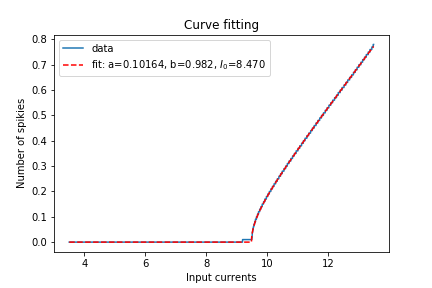
\includegraphics[width = 10 cm]{figs/Rotational/spikies_num_vs_input_fitted_curve_g50_input_3.5_13.5.png}
 \caption{تعداد تیزه بر حسب جریان تصادفی برای سامانه‌ای با ده هزار نورون و ضریب تاثیر $g=50$}
  \label{fig:spikes_num_vs_background_current}
\end{figure}

تعداد تیزه‌های کل شبکه رابطه‌ی مستقیمی با جریان خارجی جاری در شبکه دارد. می‌توانیم با محاسبات تحلیلی نیز به شکل بدست آمده از شبیه‌سازی عددی نزدیک شویم:

\begin{align}
\begin{cases}
I_{in} &= -g \int_{a_{min}}^{a_{max}} p(a) f(a + I_{in}) da \\
f(a) &= \frac{\sqrt{a^2 - 1}}{2\pi}
\end{cases}
\label{eq:analytical_input_current}
\end{align}

در رابطه \ref{eq:analytical_input_current} ، $f(a)$ تابع فعالیت (تعداد تیزه بر ثانیه) تک نورون بر حسب جریان کل ورودی آن است. همچنین $I_{in}$ تمام جریان خارجی جاری در شبکه است.\\
حل این رابطه کمی دشوار است زیرا جریان کل را بر حسب خودش محاسبه کرده است. اما از آنجایی که در انتگرال‌ده تنها یک جابجایی ثابت رخداده است؛ صورت کلی پاسخ انتگرال تغییر نمی‌کند و به صورت زیر بدست خواهد آمد.
\begin{align}
I_{in} = \frac{-g}{2} (-a \sqrt{-1 + a^2} + log(a + \sqrt{-1 + a^2})) \Big|_{a_{min} + I_{in}}^{a_{max} + I_{in}}
\end{align}
\زیرقسمت{پهن‌کردن قالی صفحه‌ی فاز}
در قسمت‌های پیشین تنها به مطالعه‌ی تاثیر ضریب اتصال در تغییرفاز پرداختیم و زمان تاخیر را تنها در $t_d = 0.1 s$ خلاصه کردیم. حال اجازه دهید تا به تاخیر نیز اجازه‌ی تغییر دهیم. در ادامه‌ی این قسمت از نوشتارمان، به فرش‌کردن صفحه‌ی فاز خود خواهیم پرداخت. امید است که چهره‌ی تمام نمای سامانه‌ بر صورت این قالی نقش بندد.\\


\زیرزیرقسمت{قالی انحراف از معیار میدان}
در شکل \ref{fig:rot_g_d_phase_space} مشاهده می‌کنیم که شدت هم‌گامی در هر کدام از هنگردهای سامانه چقدر است. بنظر می‌رسد که با افزایش زمان تاخیر و ضریب تاثیر همگامی قدرت پیدا می‌کند و هر دو در ظهور این رفتار شریک هستند.
\begin{figure}[h]
\centering
  \includegraphics[width = 15 cm]{../scripts/all_neurons_model_in_one_place/Rotational_ensembles/N10000_T100_I9.5_13.5_cluster_computed/sigma_phase_space.png}
 \caption{صفحه‌ی فاز مربوط به سامانه‌ی نورون‌های چرخنده}
  \label{fig:rot_g_d_phase_space}
\end{figure}

\قسمت{شبکه‌ نورون‌های ساده}
حل مسئله‌ی مدل چرخنده‌ بسیار دشوار است و تا تاریخ نوشتن این بند، راه‌حلی تحلیلی برای توصیف گذرفاز آن نیافته‌ایم. علت این موضوع هم حضور جمله‌ی غیرخطی $- cos(\theta)$ در جمله‌ی برهم‌کنش‌های آن‌هاست. حال که با ابعاد دشوار مسئله روبرو شده‌ایم؛ اجازه دهید که زمین بازی خود را عوض کنیم.\\
می‌پرسیم که آیا کیفیت گذرفاز از ناهم‌گامی به هم‌گامی به این جمله وابسته است؟ بی‌تردید پاسخ این سوال را نخواهیم فهمید؛ مگر آن که شبکه‌ی جدیدی مطابق درخواست خود ابداع و شبیه‌سازی کنیم.

\begin{tcolorbox}
\begin{equation}
\begin{cases}
\dot{\theta_i}=I_i  - g E, \hspace{2ex}  \theta_i \leq \pi \\
\dot{E} = M - \alpha E\\
\dot{M} = -  \alpha M + \frac{ \alpha^{2} }{N} \sum_{n|tـn<t} \delta(t - t_n - t_d)
\end{cases}
\end{equation}
\begin{enumerate}[-]
\item $\theta_i$:
مشخص کننده‌ی فاز هر نورون. این فاز میان دو لبه در حال حیات است. کوچکترین کران بالای آن همان حالت آستانه در $\pi$ است و بزرگترین کران پایین آن نگه‌دارنده‌ای است که از ریزش نورون‌ها جلوگیری می‌کند.
\item $E$:
میدانی است که شدت فعالیت شبکه را نشان می‌دهد.
\item $M$:
یک پارامتر فرعی که در حل معادله دیفرانسیل مرتبه دوم به دو معادله‌ی تحول مرتبه اول ما را یاری کرده است.
\end{enumerate}
\end{tcolorbox}

همچنین دقت کنیم که اگر چه این مدل کاهش یافته‌ای از مدل چرخنده است اما در صورت کاستن مدل انباشت‌وشلیک هم به همین جملات برهم‌کنشی می‌رسیدیم. تنها تفاوت در آن می‌شد که فاصله‌ی بین حالت تیزه ($\pi$) و بازنشانی (صفر) در حالت ابداعی $\pi$ برابر مدل کاسته‌شده‌ی انباشت‌وشلیک می‌شد.

\زیرقسمت{شبیه‌سازی}
برای مدل توصیف شده‌ی بالا شبیه‌سازی خود را با تنظیمات زیر به اجرا گذاشتیم. 
\begin{tcolorbox}[colback=green!5!white,colframe=green!75!black]
\begin{enumerate}[*]
\item
$\alpha = 20\, s^{-1}$
\item
جریان‌های تصادفی خارجی نورون‌ها از اعضای بازه‌ی $(9.5,13.5)$ انتخاب می‌شوند.
\item
$N = 10000$
\item
$t_d = 0.1\, s$ 
\end{enumerate}
\end{tcolorbox}

\زیرقسمت{نتایج}
\زیرزیرقسمت{در جستجوی تغییرفاز}
قابل توجه است که کیفیت تغییرفاز با حذف جمله‌ی ذکر شده تغییر نکرد و تنها مکان و ارتفاع انحراف از معیار جریان داخلی است که دست خور تغییر شده است - شکل \ref{fig:sigma_non_repulsive}.
\begin{figure}
\centering
  \includegraphics[width = 10 cm]{../scripts/all_neurons_model_in_one_place/Non_repulsive_rotational_ensembles/N10000_T100_I9.5_13.5/sigma_g_0.1_65.png}
 \caption{پهنای جریان یک سامانه ساده با ده هزار نورون}
  \label{fig:sigma_non_repulsive}
\end{figure}

\قسمت{تلاش برای توصیف}

از آنجا که شبیه‌سازی این سامانه شامل تعریف فرآیندهای متفاوتی بود؛ بدیهی است که نوشتن معادله‌ی تحلیلی برای توصیف کامل آن آسان نباشد. اما در این بخش تلاش می‌کنیم که با کنار هم قرار دادن معادلات اصلی چارچوب مسئله‌ی خود را مشخص کنیم.\\
هر نورون که از حالت $\theta = \pi$ عبور می‌کند [تیزه می‌زند] باعث می‌شود تا سهمی از جریان با کیفیت $p(t):= \alpha^2 t \cdot exp(-\alpha t)$ به جریان درونی کل سامانه $E(t)$ اضافه شود.
\begin{equation}
E(t) = \frac{1}{N}\int_{- \infty}^{t - d} \int J_a (\pi,u) da \cdot u\, e^{-\alpha u} du
\end{equation}
(چک شود آیا بعد معادله درست است؟)\\
اما جریان برای هر نورون با ورودی $a$ به طریق زیر است:
\begin{equation}
J_a (\theta, t) = n_a(\theta,t) \cdot \dot \theta_a
\end{equation}
این رفتار به خوبی نشان می‌دهد جریان فقط در ناحیه‌ی $\theta \leq \pi$ وجود دارد. زیرا ورود نورون به ناحیه‌ی مثبت‌تر را ممنوع کرده‌ایم.  بی‌تردید برای فهمیدن چگونگی تغییر جریان در ناحیه‌های میانی باید از معادله‌ی پخش استفاده کنیم.
\begin{align}
\frac{\partial n_a}{\partial t} &= - \frac{\partial J_a}{\partial \theta}\\
&= - \frac{\partial n_a}{\partial \theta} \cdot \dot \theta_a
\end{align}
\زیرقسمت{حل معادله‌ی شبکه‌ی ساده}
اجازه بدهید تا اولین تلاش خود را از ساده‌ترین نوع شبکه‌ها شروع کنیم. شبکه‌ای که به جز جریان داخلی و جریان تصادفی اولیه ورودی دیگری ندارد. پس خواهیم داشت:
\begin{align}
\begin{cases}
E(t) = \frac{1}{N} \int_{- \infty}^{t - d} \int n_a(\pi,u) \cdot \big[ a - g E(u) \big] da \cdot \alpha^2 u\, e^{-\alpha u} du \\
\frac{\partial n_a}{\partial t} = - \frac{\partial n_a}{\partial \theta} \cdot (a - g E(t) )
\end{cases}
\label{eq:simple_network}
\end{align}
چند پیشنهاد می‌شود برای ادامه‌ی راه‌حل داشت.
\begin{enumerate}[1.]
\item
از آنجا که میدان به گونه‌ای متناوب عمل می‌کند؛ یک پیشنهاد خوب می‌تواند آن باشد که بسط فوریه‌ی آن را بنویسیم.
\begin{equation}
E(t) = \sum c_i \cdot cos(\omega_i t)
\end{equation}
که اگر ثابت کنیم $c_1$ از بقیه ضرایب بزرگتر است؛ مساله‌ی ما حل می‌شود.
\item
دشواری مساله از در هم تنیدگی معادلات برآمده است. اگر به تقریب در معادله‌ی پخش میدان را یک نوفه درنظر بگیریم و پاسخ را در معادله‌ی اول قرار دهیم.
\item
انتگرال اول را به صورت بازگشتی در خودش جاگذاری کنیم.
\item
مسئله را در حالت آماری بررسی کنیم و حالت پایستار آن را پیدا کنیم و  بپرسیم در چه حالتی است که حالت پایستار داریم.
\end{enumerate}

\زیرزیرقسمت{روش بازگشتی}
در این روش برای این که از جمله‌ی تابعیت $E(u)$ را از خودش باز کنیم؛ عبارت سمت راست را مجددا در خودش جاگذاری می‌کنیم. برای راحت‌تر شدن محاسبات ابتدا دو متغیر کمکی زیر را تعریف می‌کنیم:
% abbrivations for calculation of this section
\newcommand{\J}[1]{\mathcal{J}(\pi,u_{#1})}
\newcommand{\N}[1]{\mathcal{N}(\pi,u_{#1})}

\newcommand{\A}[1]{\mathcal{A}(#1 - d)}

\newcommand{\impact}[1]{u_{#1}\, e^{-\alpha u_{#1}}}
%
\begin{align}
\J{} &\equiv \int n_a(\pi,u) a \cdot da\\
\N{} &\equiv \int n_a(\pi,u) \cdot da
\end{align}
عبارت $\J{}$ به معنای جمع جریان تصادفی نورون‌هایی است که در زمان u در آستانه قرار دارند. همچنین عبارت $\N{}$ به معنای تعداد همین نورون‌هاست.\\
حال با نمادهای بالا شروع به بازنویسی جملات پیشین می‌کنیم:
\begin{align}
E(t) &= \frac{1}{N} \int_{- \infty}^{t - d} \N{} \cdot u\, e^{-\alpha u} du  - \frac{g}{N}\int_{- \infty}^{t - d} \J{} \cdot u\, e^{-\alpha u} E(u)  du\\
\end{align}
حال جمله‌ی اول را نیز با عبارت دیگری خلاصه‌سازی می‌کنیم:

\begin{equation}
\A{t} \equiv \frac{1}{N}\int_{- \infty}^{t - d} \N{} \cdot u\, e^{-\alpha u} du 
\end{equation}
این عبارت جمع تعداد همه‌ی تیزه‌هایی است که تا گام $t-d$ زده شده‌اند و درنتیجه جمله‌ای انباشتی است. پس خواهیم داشت:
\begin{changemargin}{-3cm}{-3cm} 
%your text here  
\begin{align}
E(t) &= \A{t} - g\int_{- \infty}^{t - d} \J{} \cdot u\, e^{-\alpha u}E(u) du\\
&= \A{t} - g\int_{- \infty}^{t - d} \J{1} \cdot \impact{1} \cdot \big[ \A{u_1} - g\int_{- \infty}^{u_1 - d} \J{2} \cdot \impact{2} E(u_2) du_2 \big] du_1\\
&= \A{t} - g\int_{- \infty}^{t - d} \J{1} \cdot \impact{1} \cdot \A{u_1} du_1\\ 
&\hspace{1 cm}+ g^2 \int_{- \infty}^{t - d} \J{1} \cdot \impact{1}\int_{- \infty}^{u_1 - d} \J{2} \cdot \impact{2} E(u_2) du_2 du_1\\
&= \A{t} - g\int_{- \infty}^{t - d} \J{1} \cdot \impact{1} \cdot \A{u_1} du_1\\ 
&\hspace{1 cm}+ g^2 \int_{- \infty}^{t - d} \J{1} \cdot \impact{1}\int_{- \infty}^{u_1 - d} \J{2} \cdot \impact{2} \A{u_2} du_2 du_1\\
&\hspace{1 cm}- g^3 \int_{- \infty}^{t - d} \J{1} \cdot \impact{1}\int_{- \infty}^{u_1 - d} \J{2} \cdot \impact{2} \int_{- \infty}^{u_2 - d} \J{3} \cdot \impact{3} E(u_3) du_3 du_2 du_1
\end{align}

\end{changemargin}

حال در این میان دو نکته قابل توجه است. (۱) میدان در هر زمان وابسته به اثرات انباشتگی از زمان ازل سامانه است. عمر این سامانه کراندار باشد؛ تعداد جملات بالا محدود می‌شوند. (۲) دقت کنید که بازه‌ی متغیرهای انتگرال‌ده به صورت 
$- \infty \leq u_{i+1} \leq u_i - d$
محدود می‌شوند. پس طبیعی است که نتیجه بگیریم بازه‌ی هر انتگرال تو در تو چند گام عقب‌تر از زمان اکنون است. یعنی 
$- \infty \leq u_{i} \leq t - i \, d$.


\زیرزیرقسمت{روش اختلال}
به نمودار \ref{fig:sigma_rotational} دقت کنید. در زمانی که تعداد نورون‌ها بی‌نهایت باشد؛ در فاز ناهم‌گام انحراف معیار میدان صفر خواهد شد. این به این معنی است که جریان در زمان ثابت خواهد ماند. پس بگذارید با علم بر این موضوع یک جواب معادله‌ی \ref{eq:simple_network} را در حالت حدی میدان ثابت $E_0$ معرفی کنیم.\\
با فرض ثابت بودن میدان، اندازه‌ی آن را محاسبه می‌کنیم. سپس مجدد به معادلات برمی‌گردیم و می‌پرسیم که در صورت جمع با یک جمله‌ی اختلالی کوچک این انحراف رشد خواهد کرد یا خیر. به عبارت دیگر آیا این جواب جاذب است.\\
\begin{align}
\begin{cases}
E_0 = \frac{1}{N}\int_{- \infty}^{t - d} \int n_a(\pi,u) \cdot \big[ a - g E_0 \big] da \cdot \alpha^2 u\, e^{-\alpha u} du \\
\frac{\partial n_a}{\partial t} = - \frac{\partial n_a}{\partial \theta} \cdot (a - g E_0 )
\end{cases}
\end{align}

یک راه خوب برای پیشبرد سطر اول معادلات آن است که از دو طرف آهنگ تغییرشان با زمان را بپرسیم. از آنجا که سمت چپ معادله ثابت است؛ سمت راست هم باید جوابی مشابه را حکایت کند.\\
\begin{equation}
0 = \frac{dE_0}{dt} = \frac{\alpha^2 (t-d) e^{-\alpha (t-d)}}{N} \cdot [ - gE_0 \cdot \int n_a(\pi,t-d) da + \int n_a(\pi,t-d)\cdot a\,da ]
\end{equation}
مشخص است که کدام جمله از جملات ضربی بالا صفر است. پس برای $E_0$ خواهیم داشت:
\begin{equation}
E_0 = \frac{1}{g}\cdot \frac{\int n_a(\pi,t-d)\cdot a\,da}{\int n_a(\pi,t-d) da }
\end{equation}

حال برای ادامه‌ی فرآیند نیاز داریم تا عبارت حاکم بر 
$n_a(\pi,t-d)$
را بدست آوریم. جواب پیشنهادی ما برای سطر دوم معادلات از جنس تابع دلتاست:
\begin{align}
n_a(\theta,t) &= \delta(\theta - \theta_a(t)) \\
&= \delta(\theta + \theta_0 - (a - g E_0)t + 2 \floor{K^{(t)}_a}\pi )\\
&= \delta( \theta - (a - g E_0)t + 2 \floor{K^{(t)}_a} \pi + \theta_0  )\\
\Rightarrow n_a(\pi,t) &= \delta(  (2\floor{K^{(t)}_a} + 1)\pi - (a - g E_0)t + \theta_0   )\\
\end{align}
که در این معادلات 
$K^{(t)}_a$
کسری است که تعداد دور هر نورون را از آغاز تا کنون روایت می‌کند و ما مجبور به عقب کشیدن 
$2\pi$
فاز کامل پس از تیزه زدن آن به تعداد 
$\floor{K^{(t)}_a}$
شده‌ایم.
\footnote{دقت کنیم که معادله‌ی ذکر شده برای نورون‌هایی درست است که 
$(a - g E_0) > 0 $
}
  قابل محاسبه است که عبارت کامل آن به صورت زیر است.
\begin{equation}
K^{(t)}_a = \frac{(a - gE_0)t + \pi + \theta_0}{2\pi}
\end{equation}

برای محاسبه‌ی انتگرال‌هایی که شامل این دلتای دیراک هستند؛ لازم است تا صفر‌های آرگومان آن را محاسبه کنیم.
\begin{align}
\big( 2 \floor{\frac{(a - gE_0)t + \pi + \theta_0}{2\pi}} + 1 \big)\pi - (a - g E_0)t + \theta_0 &= 0\\
2\pi \times \bigg( \floor{\frac{(a - gE_0)t + \pi + \theta_0}{2\pi}}  - \frac{(a - gE_0)t + \pi + \theta_0}{2\pi} \bigg) &= 0\\
2\pi \times \bigg( \floor{K^{(t)}_a} - K^{(t)}_a \bigg) &= 0  \label{eq:neuron_pattern_simple_model}
\end{align}
این رابطه کاملا یک تابع تناوبی را توصیف می‌کند. یک تابع مقطع که در مکانی که آرگومان آن صحیح می‌شود؛ مقدار صفر به خود می‌گیرد. پس روشن است که توقع داشته باشیم. تعداد صفرهای این معادله به اندازه‌ی تعداد تناوبی است که در هر زمان در بازه‌ی جریان‌های داده شده دارد.
\begin{align}
\Delta K^{(t)}_a  &= 1\\
\Delta K^{(t)}_a &= \frac{t}{2\pi}\Delta a\\
\Delta a &= \frac{2\pi}{t}
\end{align}
این دوره‌ی تناوب با افزایش زمان کوچکتر می‌شود. اگر تعداد نورون‌ها را به صورتی ترمودینامیکی بزرگ بگیریم؛ آنگاه به ازای هر دوره‌ی تناوب یک نورون حتما هست که روی محور آستانه قرار گرفته است.\\
حال که دوره‌ی تناوب 
$\Delta a$
را بدست آوردیم؛ می‌دانیم که ریشه‌های رابطه‌ی 
\ref{eq:neuron_pattern_simple_model}
چه زمانی رخ می‌دهند. فرض کنیم که اولین صفر در جریانی مثل
$a_m$
رخ می‌دهد. توجه کنید حتما اندازه‌ی این جریان به گونه‌ای است که نورون را به صورت فعال نگه دارد. پس باید حتما
$(a_m - g E_0) > 0 $
باشد.
 حال می‌توانیم انتگرال‌های مورد نظر خود را این چنین بسط دهیم.

\begin{align}
\int n_a(\pi,t-d)a\,da &= \int \delta \bigg( 2\pi ( \floor{K^{(t)}_a} - K^{(t)}_a) \bigg) a\,da\\
&= \frac{1}{2\pi} \cdot \sum_{K^{(t)}_a \in Z} a_i \\
&= \frac{1}{2\pi} \cdot \sum^{M}_{m=0} a_m + m \cdot \Delta a\\
&= \frac{M+1}{2\pi} \cdot ( \frac{a_m +a_{max} }{2} )\\
\end{align}
و از طرفی:
\begin{align}
\int n_a(\pi,t-d)\,da &= \int \delta \bigg( 2\pi ( \floor{K^{(t)}_a} - K^{(t)}_a) \bigg) a\,da\\
&= \frac{1}{2\pi} \cdot \sum_{K^{(t)}_a \in Z} 1 \\
&= \frac{1}{2\pi} \cdot \sum^{M}_{m=0}  1\\
&= \frac{M+1}{2\pi}
\end{align}
حال اگر به محاسبه‌ی میدان ثابت خود برگردیم و تکه‌های پازل را کنار هم بگذاریم؛ خواهیم داشت:
\begin{align}
E_0 &= \frac{1}{g}\cdot \frac{\int n_a(\pi,t-d)\cdot a\,da}{\int n_a(\pi,t-d) da } \\
&= \frac{1}{g}\cdot \frac{ \frac{M+1}{2\pi} \cdot ( \frac{a_m +a_{max} }{2} ) }{ \frac{M+1}{2\pi} } \\
&= \frac{1}{g} ( \frac{a_m +a_{max} }{2} )
\end{align}

\زیرزیرقسمت{روش آماری}
در این روش فرض می‌کنیم که برای هر جریان تصادفی اولیه، نورون‌های زیادی را به اختیار گرفته‌ایم. در حالت پایا  ، در یک حالت خاص تغییری در چگالی جمعیت مشاهده نمی‌شود پس در معادله‌ی
\ref{eq:simple_network}
خواهیم داشت:
\begin{equation}
\frac{\partial n_a}{\partial t} = 0
\end{equation}
همچنین در حالت پایا که در واقع از نگاه ما حالت ناهم‌گام است؛ جریان بین نورون‌ها - که کمیتی بزرگ مقیاس است -  در زمان تغییری نمی‌کند. پس به این ترتیب:

\begin{align}
\begin{cases}
\frac{\partial n_a}{\partial t} = - \frac{\partial J_{a}(t)}{\partial \theta} = 0\\
J_{a}(\theta, t) = n_a(\theta,t) \cdot [ a - g E ]\\
\end{cases}
\Rightarrow J_{a}(\theta, t) = J_{a}(t)\\
\Rightarrow n_{a}(\theta, t) = n_{a}\\
\end{align}

پس توزیع جمعیت نورون‌‌ها مستقل از زمان و حالت آن‌ها خواهد شد. اگر توزیع را در ابتدا یکنواخت میان جریان‌های مختلف توزیع کرده باشیم؛ برای همه‌ی زمان‌ها و حالت‌ها داریم:
\begin{equation}
n = \frac{N}{2 \pi (a_{Max} - a_{min}) }
\end{equation}


برای جریان بین نورون‌ها هم خواهیم داشت:
\begin{align}
E &= \frac{1}{N} \int_{- \infty}^{t - d} \int n \cdot \big[ a - g E \big] da \cdot \alpha^2 u\, e^{-\alpha u} du\\
&=  \int \frac{n}{N} \cdot \big[ a - g E \big] da \label{eq:e_sum_simple}
\end{align}
دقت کنیم که انتگرال رابطه‌ی \ref{eq:e_sum_simple} روی  نورون‌هایی است که مستعد تیزه زدن هستند.
\footnote{
$(a - g E) > 0 $
}

اولین جریانی که نورون را مستعد تیزه زدن می‌کند $a_*$ نام‌گذاری می‌کنیم. محاسبات را ادامه می‌دهیم:
\begin{align}
E &=  \int \frac{n}{N} \cdot \big[ a - g E \big] da \\
&= \frac{n}{N} \cdot \big[ \frac{a^2_{Max} - {a_*}^2}{2} - g E (a_{Max} - a_*) \big] \\
\Rightarrow E &= n \cdot \big[ \frac{a^2_{Max} - {a_*}^2}{2}  \big] / \big[ N + g n (a_{Max} - a_*)\big]
\end{align}
شاید بنظر این یک معادله‌ی درجه یک ساده باشد که میدان را گزارش می‌کند اما در واقع خود $a^*$ هم به میدان وابسته است و باید وابستگی آن را لحاظ کنیم. به تقریب:
$a^{*} = gE$
با اضافه کردن این معادله و حل معمول یک معادله‌ی درجه‌ی دو برای میدان صراحتا خواهیم داشت:
\begin{align}
E =  \big( \frac{a_{Max}}{g} + \frac{N}{n g^2}  \big) \pm \big[ \big( \frac{N}{n g^2} + \frac{a_{Max}}{g} \big)^2 - \frac{{a_{Max}}^2}{g^2} \big]^{\frac{1}{2}}
\end{align}
نتیجه می‌دهد که $a_{*}$ هم باید به صورت زیر باشد:
\begin{align}
a_{*} &=  \big( a_{Max} + \frac{N}{n g} \big) \pm \big[ \big( \frac{N}{n g} + a_{Max} \big)^2 - {a_{Max}}^2 \big]^{\frac{1}{2}}\\
&=  \big( a_{Max} + \frac{N}{n g} \big) \pm \big[  \frac{N^2}{n^2 g^2} + \frac{2a_{Max}}{ng}  \big]^{\frac{1}{2}}
\end{align}
اجازه بدهید علامت مثبت را کنار بگذاریم زیرا مقدار $a_{*}$ را خارج بازه‌ی جریان‌های سامانه گزارش می‌کند. پس هم برای میدان و هم جریان $a_{*}$ خواهیم داشت:
\begin{align}
\begin{cases}
a_{*} =  \big( a_{Max} + \frac{N}{n g} \big) - \big[  \frac{N^2}{n^2 g^2} + \frac{2a_{Max}}{ng}  \big]^{\frac{1}{2}}\\
E =  \big( \frac{a_{Max}}{g} + \frac{N}{n g^2} \big) - \big[ \frac{N^2}{n^2 g^4} + \frac{2Na_{Max}}{ng^3}  \big]^{\frac{1}{2}}\\
\end{cases}
\end{align}
در ضریب تاثیرهای بسیار بزرگ داریم:(اشتباه است تصحیح شود.)
\begin{align}
E \cong & \frac{a_{Max}}{g} + \frac{N}{ng^2} - (\frac{2N a_{Max}}{n g^3})^{\frac{1}{2}} \big[ 1 + \frac{N}{2nga_{Max}} \big]^{\frac{1}{2}}\\
=& \frac{a_{Max}}{g} + \frac{N}{ng^2} - (\frac{2 N a_{Max}}{n g^3})^{\frac{1}{2}} \big[ 1 + \frac{N}{4nga_{Max}} \big]\\
=& \frac{a_{Max}}{g} - (\frac{2 N a_{Max}}{n g^3})^{\frac{1}{2}} + \frac{N}{ng^2}  - (\frac{N}{2n})^{\frac{3}{2}}  \cdot \frac{1}{ {a^{\frac{1}{2}}_{Max} g^{\frac{5}{2}}}}
\end{align}

\subsubsection{میانگین زمانی میدان}
اگر چه محاسبه‌ی انحراف معیار میدان در طول زمان کار دشواری است اما محاسبه‌ی میانگین آن نسبتا ساده‌تر است. زیرا برای هر تابع f وابسته به زمان داریم
\begin{align}
I[f] &= \lim_{T\to\infty} \frac{1}{T - d} \int^{T}_{d} dt \int_{0}^{t - d} f(u)du \\
&= \lim_{T\to\infty} \frac{1}{T - d} \int_{0}^{T - d} du \int^{T}_{u+d} f(t) dt \\
&= \lim_{T\to\infty} \int_{0}^{T - d} du \bar{f}(u)  
\end{align}
به شرط تعادل
\newpage
\bibliographystyle{plain-fa}
\bibliography{MyReferences}

\end{document}


